\section[Robustness]{Robustness of the DTR for subgroups of data}
\label{sec:robustness}


The mathematical derivation of uncertainty is to complex for this internship.
To gain a sense of how reliable the effect of DTR change is, we compare the 
results of the left and right hemisphere  -- the hemisphere from -180 to 0 and 0 to 180 degrees -- and further latitude subsets. 

\begin{figure}[ht]
    \centering
    \begin{subfigure}{0.48\textwidth}
        \centering
        \includegraphics[width = \textwidth]{C:/Users/leonh/Desktop/Praktikum_AWI/NordPolLinks/Lon_66_70/Fit/DTRperMonth.png}
    \end{subfigure}%
    \begin{subfigure}{0.48\textwidth}
        \centering
        \includegraphics[width = \textwidth]{C:/Users/leonh/Desktop/Praktikum_AWI/NordPolRechts/Lon_66_70/Fit/DTRperMonth.png}
    
    \end{subfigure}

    \begin{subfigure}{0.48\textwidth}
        \centering
        \includegraphics[width = \textwidth]{C:/Users/leonh/Desktop/Praktikum_AWI/NordPolLinks/Lon_70_75/Fit/DTRperMonth.png}
    \end{subfigure}%
    \begin{subfigure}{0.48\textwidth}
        \centering
        \includegraphics[width = \textwidth]{C:/Users/leonh/Desktop/Praktikum_AWI/NordPolRechts/Lon_70_75/Fit/DTRperMonth.png}
    \end{subfigure}

    \begin{subfigure}{0.48\textwidth}
        \centering
        \includegraphics[width = \textwidth]{C:/Users/leonh/Desktop/Praktikum_AWI/NordPolLinks/Lon_75_80/Fit/DTRperMonth.png}
    \end{subfigure}%
    \begin{subfigure}{0.48\textwidth}
        \centering
        \includegraphics[width = \textwidth]{C:/Users/leonh/Desktop/Praktikum_AWI/NordPolRechts/Lon_75_80/Fit/DTRperMonth.png}
    \end{subfigure}
    
    \begin{subfigure}{0.48\textwidth}
        \centering
        \includegraphics[width = \textwidth]{C:/Users/leonh/Desktop/Praktikum_AWI/NordPolLinks/Lon_80_84/Fit/DTRperMonth.png}
    \end{subfigure}%
    \begin{subfigure}{0.48\textwidth}
        \centering
        \includegraphics[width = \textwidth]{C:/Users/leonh/Desktop/Praktikum_AWI/NordPolRechts/Lon_80_82/Fit/DTRperMonth.png}
    \end{subfigure}

    \caption{Subfigure with Two Columns}
    \label{fig:DTRleftright}
\end{figure}

% As can be seen in \cref{fig:DTRleftright}, the DTR differs significantly, especially for higher Breitengrade. This may be caused by the 
% selection of data. The data covers the area represented in \cref{fig:datacoverage}. When splitting the data in the 
% left an right hand side, the landmass is not divided equally, but the left half of the earth contains mainland, whereas the right hemisphere contains islands. Therefore the 
% temperatures differ significantly, as on the islands e.g the formation of ice plays a role. 

As depicted in Figure \ref{fig:DTRleftright}, the Diurnal Temperature Range (DTR) exhibits significant variations, particularly at higher
latitudes. This variability may be attributed to the data selection process. The dataset encompasses the geographic region illustrated
in Figure \ref{fig:datacoverage}. When segregating the data into left and right hemispheres, it becomes apparent that the distribution
of landmass is uneven. The left half of the Earth predominantly comprises mainland, whereas the right hemisphere consists mainly of islands.
Consequently, temperature variations are influenced by the geographical circumstances, with islands experiencing unique factors such as ice
formation, which influence their climate differently.

As shown in \cref{app:MaxTemp,app:MinTemp}, the temperatures and their trends differ significantly for the two areas. The mainland experiences 
lower temperatures than the island dominated areas, especially for the areas of higher latitude. To check wether the data is robust, we have to compare two equivalent 
areas. Therefore, Greenland is divided into two halfs and the process is repeated. 




\begin{figure}[h]
    \centering
    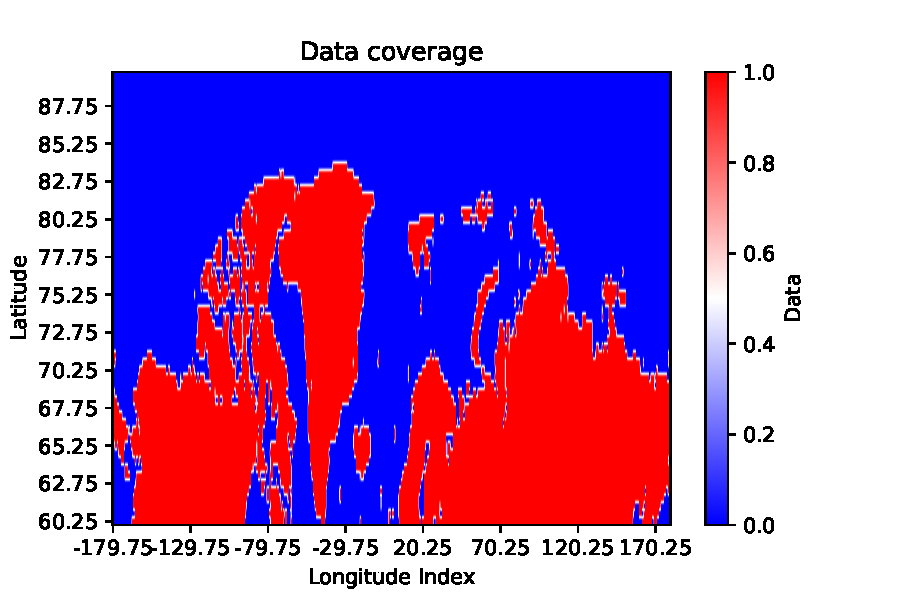
\includegraphics[width = 12cm]{C:/Users/leonh/Desktop/Praktikum_AWI/datacoverage.pdf}
    \caption[short]{Data coverage of the CRU data.}
    \label{fig:datacoverage}
\end{figure}